\documentclass{article}
\usepackage{tikz,lipsum,lmodern}
\usepackage[most]{tcolorbox}
\usepackage[paperheight=10.75in,paperwidth=7.25in,margin=1in,heightrounded]{geometry}
\usepackage{graphicx}
\usepackage{blindtext}
\usepackage{ragged2e}
\usepackage[space]{grffile}

%\graphicspath{{"/home/silasUser/Documents/testDir/with blank/"}}
\graphicspath{{"/home/silasUser/.local/share/Anki2/User 1/collection.media/"}}

\title{todo extract deck name}

\begin{document}
%*********************
\section{Generelles}
%---------------------
\begin{tcolorbox}[colback=white!10!white,colframe=lightgray!75!black,
  savelowerto=\jobname_ex.tex]

\begin{center}
 Erläutern Sie die Motivation hinter der Datenbanktheorie. Gehen Sie insbesondere auf die 
Probleme ein, und beschreiben Sie was es heißt wenn ein Datum integer

\end{center}

\tcblower

\justifying

%\includegraphics{/home/silasUser/.local/share/Anki2/User 1/collection.media/test.PNG}
\includegraphics{test.PNG}
\end{tcolorbox}

\end{document}


